% Beamer slide template prepared by Tom Clark <tom.clark@op.ac.nz>
% Otago Polytechnic
% Dec 2012

\documentclass[10pt]{beamer}
\usetheme{CambridgeUS}
\usepackage{graphicx}
\usepackage{fancyvrb}

\newcommand\codeHighlight[1]{\textcolor[rgb]{1,0,0}{\textbf{#1}}}

\title{A Quick Introduction to BSD}

\author[IN715]{Networks Three}
\institute[Otago Polytechnic]{
  Otago Polytechnic \\
  Dunedin, New Zealand \\
}
\date{}
\begin{document}

%----------- titlepage ----------------------------------------------%
\begin{frame}[plain]
  \titlepage
\end{frame}



%----------- frame  ----------------------------------------------%
\begin{frame}
  \frametitle{BSD}
  \begin{itemize}
    \item In this paper we will use BSD Unix for some of our work.
    \item Most of you are familiar with Linux.  BSD is very similar.
    \item Despite its similarity to Linux, there is some value in 
          introducing you to another system.
    \item BSD has some properties that are very desirable for 
          network infrastructure services.
  \end{itemize}  
\end{frame}

%----------- frame  ----------------------------------------------%
\begin{frame}
    \begin{figure}[h!]
    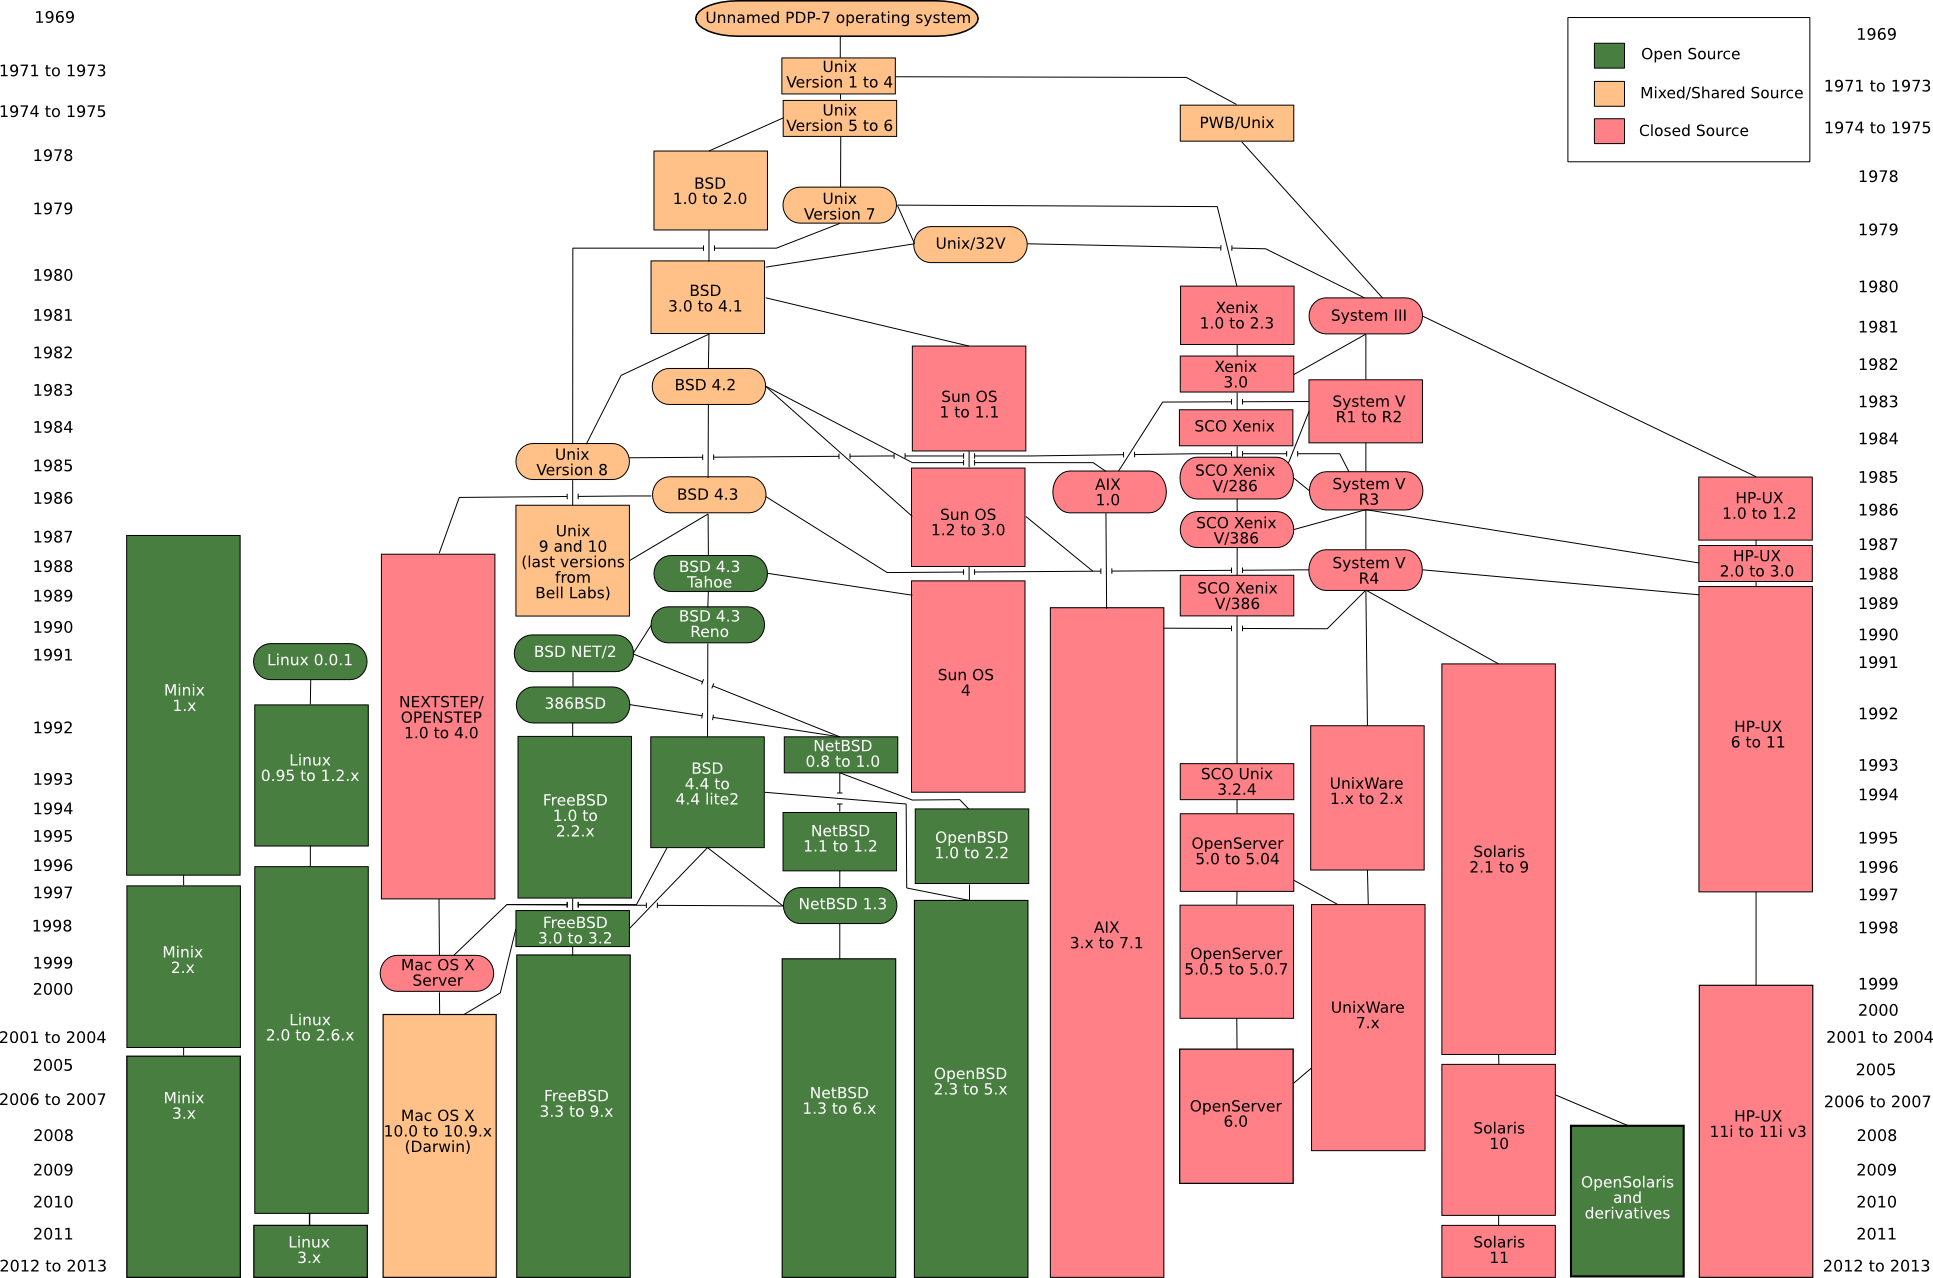
\includegraphics[scale=0.15]{unix-history.png}

\caption{``Unix history-simple" by Eraserhead1, Infinity0, Sav\_vas - Levenez Unix History Diagram, Information on the history of IBM's AIX on ibm.com. Licensed under Creative Commons Attribution-Share Alike 3.0 via Wikimedia Commons}
    \end{figure}
\end{frame}


%----------- frame  ----------------------------------------------%
\begin{frame}
  \frametitle{A little history}
  \begin{itemize}
    \item Unix was originally developed at Bell Labs (AT\&T).
    \item In the 1970s it was distributed as source code.  It
          was not uncommon for users to modify the source to produce
          custom versions.
    \item Some of the popular customisations were distributed as patches.
    \item BSD got its start as a collection of patches.
  \end{itemize}  
\end{frame}

%----------- frame  ----------------------------------------------%
\begin{frame}
  \frametitle{A little history}
  \begin{itemize}
    \item In the early 1990s BSD was involved in copyright troubles with
          AT\&T for distributing its code along with BSD.
    \item Eventually the dispute was resolved in 1994.  AT\&T code was
          replaced by unencumbered versions.
    \item But in the meantime, Linus Torvalds had released early versions
          of Linux.
  \end{itemize}  
\end{frame}


%----------- frame  ----------------------------------------------%
\begin{frame}
  \frametitle{BSD vs. Linux}
  \begin{itemize}
    \item Today Linux is the dominant Unix-like\footnote{Linux is extremely similar to Unix, but it is not technically Unix.} operating system.
    \item BSD systems are still widely used, however.
    \item In comparison to Linux, BSD is a little more ``old school".  While
          it lags behind Linux in terms of some features, it is widely 
          regarded as more stable and easy to maintain.
  \end{itemize}  
\end{frame}


%----------- frame  ----------------------------------------------%
\begin{frame}
  \frametitle{Types of BSD}
  Like Linux, there are many varieties of BSD the three most notable are
  \begin{itemize}
    \item FreeBSD, a widely used general purpose version
    \item NetBSD, a version focused on portability
    \item OpenBSD, a version focused on security
  \end{itemize}  

  All of these are Free/Open Source.
\end{frame}


%----------- frame  ----------------------------------------------%
\begin{frame}
  \frametitle{Configuration differences}
  \begin{itemize}
    \item The process for configuring BSD systems is very similar
          to the one for Linux.
    \item Config files are generally under /etc.
    \item The config file formats for 3rd party software is generally the same.
    \item Some config files, like those for starting/stopping services, are
          a bit different.
  \end{itemize}  
\end{frame}



%----------- frame  ----------------------------------------------%
\begin{frame}
  \frametitle{Package management}
  \begin{itemize}
    \item BSD systems use two parallel package management systems: Packages and Ports.
    \item Packages are prebuilt binaries.
    \item Ports are distributed as source code which is compiled on your
          system at install time.
  \end{itemize}  
\end{frame}

%----------- frame  ----------------------------------------------%
\begin{frame}
  \frametitle{In conclusion}

   When the most important properties in a server are reliability and
   security, then on of the BSD versions is a good choice.  You won't 
   have some of the shiny new tools that are available on a system like Linux,
   but for network infrastructure this is not a bad thing.
\end{frame}
\end{document}
